%% PARTIE 3 : Méthodologie et outils de développement

\subsection{Méthode Kanban}

La réalisation du projet a été faite en suivant la méthode Kanban, une méthode agile et itérative. La méthode consiste notamment à représenter les tâches composant le projet sur un tableau en plusieurs colonnes afin que tous les participants puissent suivre l'avancement de ce dernier.\\

Comme plusieurs autres méthodes agiles, elle repose sur le concept d'\textit{User Story} (U.S.). Cette expression désigne un besoin exprimé du point de vue du client, qu'on peut mettre sous la forme \textit{En tant que [...], je veux [...] afin de [...]}, que le développeur est chargé de réaliser.\\

Le fait de représenter l'ensemble des tâches à réaliser par le développeur sous forme d'U.S. impose de toujours voir le projet du point de vue du client, ce qui permet de rester pertinent sur ce qui est développé. Une U.S. commence à l'extrémité gauche du tableau, et se déplace vers la droite au fur et à mesure qu'elle passe les différentes étapes de réalisation, pour finir à l'extrémité droite lorsqu'elle est validée (indépendemment de ses opinions politiques).\\

La méthode Kanban, à l'inverse d'une méthode comme SCRUM, ne fonctionne pas par cycles mais en flux tendu : au lieu d'avoir un certain nombre d'U.S. à réaliser toutes les $x$ semaines, on se fixe un nombre minimal et maximal d'U.S. qui doivent être en cours de réalisation à tout moment. Ces nombres sont choisis en fonction de la capacité de travail de l'équipe de développement.\\

De plus, à toute U.S. doit être attribuée une difficulté de réalisation ainsi qu'une valeur client (utilité), qui sont des valeurs sur une échelle de Fibonacci (puisqu'il est contre-productif d'être extrêmement précis dessus). On utilise alors ces deux valeurs pour déterminer quelles U.S. réaliser parmi celles qui sont spécifiées, en prenant par exemple celles qui ont le plus grand ratio \textit{utilité/difficulté}.\\

Nous avons choisi de mettre dans notre tableau les colonnes suivantes (entre autres) :
\begin{itemize}
    \item \textbf{Product backlog} : c'est ici qu'apparaissent toutes les U.S. du projet à leur création, ainsi que les idées d'ordre plus général, issues de divers brainstorming.
    
    \item \textbf{U.S. "INVEST"} : recense toutes les U.S. mises au format "INVEST" : pour chacune, des niveaux de difficulté technique et de valeur marchandes ont été déterminés. C'est donc la liste des U.S. normalisées à faire, susceptibles de passer à la réalisation.
    
    \item \textbf{U.S. en cours} : liste les U.S. en cours de réalisation. Le nombre d'U.S. dans cette colonne est limité afin de ne pas surcharger les collaborateurs du projet. Chaque U.S. doit à ce niveau là être attribuée à une partie de l'équipe.
    
    \item \textbf{Révision} : contient les U.S. dont l'implémentation est finie mais à faire réviser par d'autres membres de l'équipe pour la logique, la lisibilité, les commentaires et plus généralement la qualité du code écrit.
    
    \item \textbf{Démo} : stocke les U.S. validées par l'équipe mais pas encore par le client. C'est la dernière étape avant qu'une U.S. soit définitivement réalisée et archivée.
\end{itemize}
Nous avons exploité le site \textit{kanboard.ipb.fr} pour travailler sur ce tableau, dont un peu voir un aperçu en figure~\ref{fig:kanboard}.

\begin{figure*}[!htb]
    \centering
    \begin{subfigure}{.8\linewidth}
        \centering
        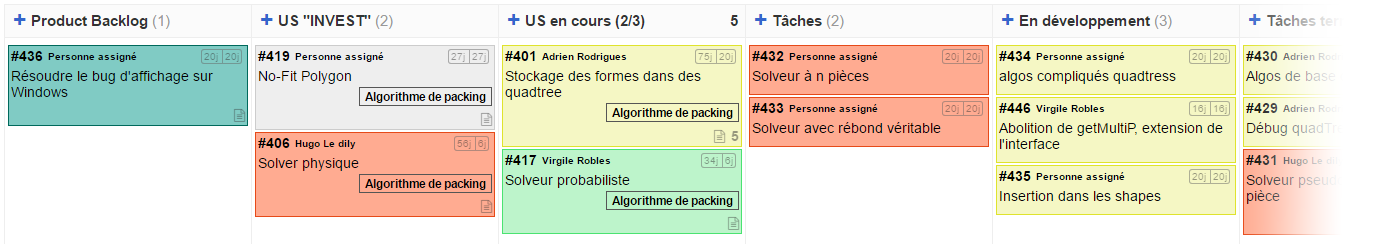
\includegraphics[width=\linewidth]{img/kanboard01.png}
    \end{subfigure}%
    ~ \\
    \begin{subfigure}{.8\linewidth}
        \centering
        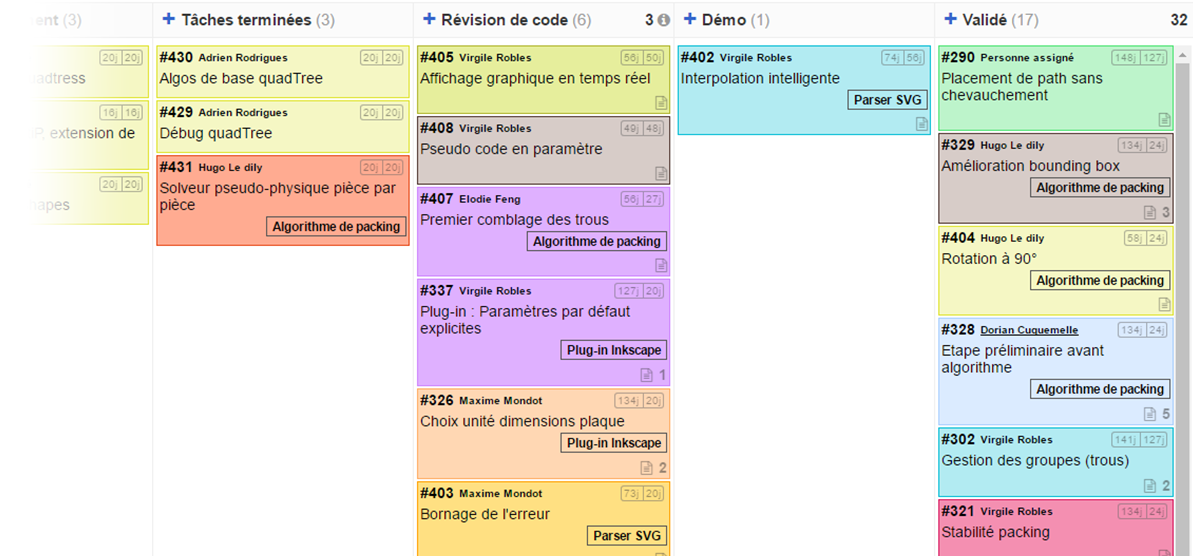
\includegraphics[width=\linewidth]{img/kanboard02.png}
    \end{subfigure}
    \caption{Aperçu de notre Kanboard}
    \label{fig:kanboard}
\end{figure*}


\subsection{La méthode dans les faits}

L'organisation du travail en équipe s'est déroulée comme suit:
\begin{itemize}
    \item A chaque réunion avec le client et/ou le responsable pédagogique, nous présentions notre travail hebdomadaire, avec démonstration d'une exécution fonctionnelle lorsque cela s'avérait pertinent.
    \item A l'issue de la réunion, nous organisions les nouvelles tâches à réaliser sous forme de nouveaux éléments dans le product backlog et d'User Stories dans notre Kanban.
    \item Ensuite, les membres de l'équipe s'accordaient à travailler en petits groupes sur plusieurs nouvelles U.S., ou continuaient à travailler sur celles qui n'avaient pas été complétées lors de la semaine.\\    
\end{itemize}

Nous avons apprécié la méthode Kanban car l'agilité nous a permis de confronter régulièrement notre avancement avec les besoins du client et ainsi de mettre à jour les attentes prioritaires, de prendre en compte ses remarques vis à vis de notre vision du sujet pour éviter les mauvaises interprétations etc.\\

%METTRE LES PROBLEMES PLUS TARD QUAND MEME...

% 1. Pourquoi ca a pas marché
% 2. Qu'est ce qu'on changerait si on devait refaire 

Nous avons cependant eu quelques légers problèmes de travail en équipe.\\

Conserver une bonne méthodologie, particulièrement pour ce qui est d'une mise-à-jour régulière du Kanban, a parfois été négligé par certains aspects : Les membres de l'équipe communiquant sur l'avancement du projet en dehors des U.S. du Kanboard, ce dernier pouvait ne pas être mis à jour systématiquement. Cet écart à la méthode s'est également manifesté par l'abandon de l'attribution des business value et des difficultés aux User Stories, la perte de la division des U.S. en tâches et la création d'U.S. de manière mal organisée.\\

De plus, le PFA était un projet réalisé en \texttt{C++}, langage appris en même temps que le début du projet. La différence d'expérience en programmation des différents membres de l'équipe se ressentait sur la contribution sur le travail au départ, car certaines personnes étaient déjà habituées à ce langage, et d'autres non.\\

Plus précisément, l'environnement de développement du projet ne favorisait pas celui-ci. En effet, dans le contexte de notre formation, nous avions de nombreux autres projets et examens, nous empêchant de nous consacrer à ce travail aussi régulièrement que l'exige la méthode. Cela met en valeur un problème intrinsèque du PFA : effectuer un travail d'entreprise dans un contexte d'école d'ingénieurs. Il est impossible de se réunir tous les matins pour faire le point sur l'avancement de chacun, de travailler en pair-programming du fait de la différence des emplois du temps de chacun etc.\\

Dans une autre mesure, il s'agissait pour tous de notre première expérience dans un projet à long terme, et avec une équipe aussi grande. La communication est un aspect essentiel au bon fonctionnement d'un projet. Mais, par manque de savoir-faire, celle-ci a parfois était imparfaite, si bien que cela a pu nous ralentir, voire empêcher la compréhension mutuelle. \\ 

%Application du Kanban
%Diff d'experience code des membres
%Première experience grand projet
%Adaptation PFA dans le cadre de l'école : réunions régulières, examens, autres projets
%...

Ces problèmes de gestion d'équipe rencontrés nous ont permis de mieux comprendre l'importance de certains points. Si nous avions à refaire ce projet, nous chercherions une méthodologie plus adaptée à l'école, ou encore à adapter une certaine méthode à cet environnement, de sorte à garantir assez de rigueur pour un meilleur travail d'équipe. Le rôle du Scrum Master, membre de l'équipe chargé d'assurer l'application de la méthode par tous les membres, a été envisagé mais jamais mis en place. Il serait donc intéressant de revoir la structuration de l'équipe (un Scrum Master fixe ou à tour de rôle). La rétrospective hebdomadaire, réunion portant sur la méthode et non sur le projet en lui-même qui vise à déterminer ce qui fonctionne et ne fonctionne pas, et à trouver des solutions sous forme de plan d'action, pourrait également être mise en place, pour une amélioration continue de notre façon de travailler.\\


%La responsabilité de répartir le travail et de former les binômes a été, sur certaines occasions, laissée aux membres les plus inspirés quant à une U.S., les autres membres assistant ces développements.\\


%Enfin, les périodes de l'année chargées en examens ont fait quelque peu fluctuer le degré d'implication dans le PFA.\\

%Au début du PFA, il y a eu un problème principalement par rapport au niveau des membres en programmation et leur degrés de maîtrise du C++. Ce qui fait qu'il fut plus difficile pour certain de suivre la cadence. Cela s'est arrangé plus tard, lorsque on a avait fini les cours et TD en C++, et lorsque les membres les plus impliqués dans le code ont baissé un peu le rythme, et ont assuré des révisions de codes pour que tout le monde soit sur la même longueur d'onde.



\subsection{Outils}
Les outils utilisés pour la réalisation du produit sont :
\begin{itemize}
    \item Langage d'extension Inkscape
    \item Python : langage de programmation utilisé pour l'interface entre Inkscape et le solveur.
    \item C++ : langage de programmation pour le solveur
    \item CMake : outil permettant de gérer la compilation et l'installation des sources.
    \item Boost : ensemble de bibliothèques C++ utilisé ici pour parser les options passées au solveur
    \item svgpp : bibliothèque aidant au parsing de fichiers SVG
    \item rapidXML : bibliothèque de parsing de fichiers XML
    \item Doxygen : permet de générer la documentation à partir des commentaires sur les sources du produit
    \item mingw-w64 : ensemble d'outils permettant la cross compilation du produit pour Windows depuis Linux.
    
\end{itemize}

\vspace{1em}
Il a été choisi de développer le produit sur Linux à l'aide de la collection de compilateurs GCC. Les plates-formes supportées sont Windows et Linux, les deux devant être compilées depuis Linux.

\subsection{Le format SVG}

\indent Les données représentant les formes à packer sont décrites sous le format SVG qui est une spécialisation du format XML. Ce format représente une arborescence de données utilisant des balises.\\

Un noeud est délimité par une balise ouvrante et une fermante, ou bien une balise seule. La balise peut contenir un ensemble d'attributs dépendant de son type. Si le noeud est sous la forme de balises ouvrantes/fermantes, il peut y avoir d'autres noeuds entre ces balises (ce sont alors des noeuds fils).\\
Un ensemble particulier de noeuds et d'attributs est utilisé lors de notre programme (un exemple de syntaxe SVG est visible en figure~\ref{fig:svg}.

\begin{itemize}
    \item \textbf{Paths} : Les \textit{paths}, et primitives de formes (\texttt{rectangle}, \texttt{circle}, ...). Ce sont les noeuds qui sont utilisés pour représenter un contour. Ils possèdent un attribut \texttt{d} qui contient l'ensemble des informations permettant de décrire ce contours, sous différentes formes : segments, courbes de Bézier, etc.
    \item \textbf{Matrices de transformations} Ce sont des attributs qui sont appliqués au \textit{path} du noeud courant ainsi que tous ses fils. Elles permettent de déplacer un objet sans modifier explicitement les coordonnées de ses points. Elles doivent donc être prises en compte lors de la lecture du fichier. Nous les utilisons également pour appliquer les déplacement effectués par le programme dans le fichier de sortie.
    \item \textbf{Groupes} : Ils forment des ensembles d'objets qui peuvent se comporter comme une entité unique, et sont particulièrement utilisés pour la gestion des formes à trous ou lors de la génération du fichier de sortie (pour délimiter les différentes plaques).
    \item \textbf{Identifiants} : Les noeuds possèdent généralement un attribut \texttt{ID}. Ils permettent d'identifier rapidement un objet, chaque objet ayant une valeur unique pour cet attribut. Celui-ci peut être modifié lors de la génération du fichier de sortie en cas de duplication des objets.
    \item \textbf{Width}/\textbf{Height}/\textbf{Viewbox} : Ce sont des attributs propre au fichier. Ils sont utilisés pour déterminer les dimensions d'une plaque par défaut, ils peuvent être exprimés dans différentes unités, qu'il nous faut donc convertir au préalable dans une unité universelle utilisable par le programme.
\end{itemize}

\begin{figure}[H]
\centering
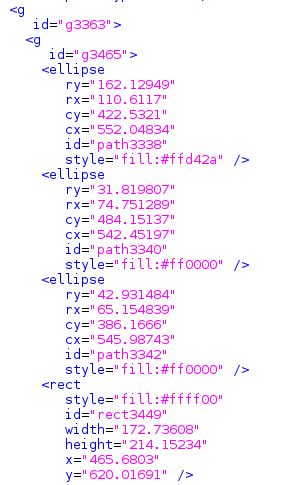
\includegraphics[scale=0.6]{img/svg.png}
\caption{Un morceau de fichier SVG}
\label{fig:svg}
\end{figure}

